% -------------------------------------------------------------------
% Thesis Template
%
% LS IV
% -------------------------------------------------------------------\\

% Personal information
\newcommand \Autor{Hendrik Rassmann}
\newcommand \Titel{Simulation eines Rechenclusters}
\newcommand \Untertitel{Bachelorarbeit}
%other information
\newcommand{\Supervisor}{Prof. Dr. Peter Bucholz\xspace}
\newcommand{\otherSupervisor}{Dr. Falko Bause\xspace}
\newcommand{\Faculty}{Fakult''at f''ur Informatik\xspace}
\newcommand{\Department}{Lehrstuhl 4\xspace}
\newcommand \Date{September 2020}

% -------------------------------------------------------------------
% Abkuerzungen formatieren %
\newcommand{\tu}{TU Dortmund\@\xspace}

\newcommand{\vgl}{vgl.\@\xspace} 
\newcommand{\Vgl}{Vgl.\@\xspace}
\newcommand{\zB}{\mbox{z.\,B.}\xspace}
\newcommand{\idR}{\mbox{i.\,d.\,R.}\xspace}
\newcommand{\bzw}{bzw.\@\xspace}
\newcommand{\dahe}{\mbox{d.\,h.}\xspace}
\newcommand{\etc}{etc.\@\xspace}
\newcommand{\evtl}{evtl.\@\xspace}
\newcommand{\ggf}{ggf.\@\xspace}
\newcommand{\bzgl}{bzgl.\@\xspace}
\newcommand{\gdw}{gdw.\@\xspace}
\newcommand{\soben}{s.\nolinebreak[4]\hspace{0.125em}\nolinebreak[4]o.\@\xspace}
\newcommand{\sunten}{s.\nolinebreak[4]\hspace{0.125em}\nolinebreak[4]u.\@\xspace}
\newcommand{\iA}{i.\nolinebreak[4]\hspace{0.125em}\nolinebreak[4]A.\@\xspace}
\newcommand{\sa}{s.\nolinebreak[4]\hspace{0.125em}\nolinebreak[4]a.\@\xspace}
\newcommand{\ua}{u.\nolinebreak[4]\hspace{0.125em}\nolinebreak[4]a.\@\xspace}
\newcommand{\og}{o.\nolinebreak[4]\hspace{0.125em}\nolinebreak[4]g.\@\xspace}
\newcommand{\oBdA}{o.\nolinebreak[4]\hspace{0.125em}\nolinebreak[4]B.\nolinebreak[4]\hspace{0.125em}d.\nolinebreak[4]\hspace{0.125em}A.\@\xspace}
\newcommand{\OBdA}{O.\nolinebreak[4]\hspace{0.125em}\nolinebreak[4]B.\nolinebreak[4]\hspace{0.125em}d.\nolinebreak[4]\hspace{0.125em}A.\@\xspace}

% ----------------------------------------------------------------------
% Start Document
% ----------------------------------------------------------------------
\documentclass[ twoside,openright,titlepage,fleqn,pointlessnumbers,headinclude, 
                11pt,a4paper,footinclude,cleardoubleempty,abstractoff
                ]{scrreprt}

% Add Packages
% -------------------------------------------------------------------
% URLs
\usepackage{url}

% -------------------------------------------------------------------
% Misc Utility
\usepackage[cmex10]{amsmath}
\usepackage[ruled,linesnumbered]{algorithm2e}
%\usepackage{algorithmicx}
\usepackage{array}
\usepackage{mdwmath}
\usepackage{mdwtab}
\usepackage{eqparbox}

% -------------------------------------------------------------------
% Grafikpakete einbinden
\usepackage{amssymb}
\usepackage{flafter}
\usepackage{listings}
\usepackage{subfig}


% -------------------------------------------------------------------
% Korrekte Darstellung der Umlaute
\usepackage[T1]{fontenc}
\usepackage{ae,aecompl}
\usepackage[utf8]{inputenc}
\usepackage[english,german,ngerman]{babel}
\usepackage{microtype}
	
% -------------------------------------------------------------------
% Anführungszeichen
\usepackage[babel,german=quotes]{csquotes}

%Grafiken ungefähr im selben bereich
\usepackage{placeins}

% Classic thesis:
\usepackage{classicthesis-ldpkg} 
% Options for classicthesis.sty:
\usepackage[eulerchapternumbers,subfig,eulermath,pdfspacing,parts,dottedtoc]{classicthesis}

% -------------------------------------------------------------------
% Setup and Finetuning
\newlength{\abcd} % for ab..z string length calculation
\newcommand{\myfloatalign}{\centering} % how all the floats will be aligned
\setlength{\extrarowheight}{3pt} % increase table row height

% -------------------------------------------------------------------
%Equation and figure numbering
\numberwithin{equation}{section} 
%sets equation numbers <chapter>.<section>.<index>
\numberwithin{table}{section} 
%sets equation numbers <chapter>.<section>.<index>
\numberwithin{figure}{section} 
%sets figure numbers <chapter>.<section>.<index>

% -------------------------------------------------------------------
% Captions look and feel
\captionsetup{format=hang,font=small}


% -------------------------------------------------------------------
% TikZ
\usepackage{tikz}
\usetikzlibrary{automata, positioning, arrows}
\usepackage{pgfplots}
\usepackage{graphicx}
\usepackage{caption}
\usepackage{subfig}
%\usepackage{subcaption}

\pgfplotsset{%
	plotstyle-unten/.style={%
		grid=major, 
		grid style={dotted,gray!25}, % Set the style
		xlabel={Deskriptorgröße $g$}, 
		ylabel={mAP [\%]},
		%every node near coord/.style={font=\footnotesize},
		legend style=
		{at={(0.5,-0.2)},anchor=north,legend columns=-1,column sep=1ex,font=\small} % Put the legend below the plot
	}
}


\pgfplotsset{%
	plotstyle-neben/.style={%
		grid=major, % Display a grid
		grid style={dashed,gray!30}, % Set the style
		%width=0.7\textwidth,
		%height=0.525\textwidth,
		%label style={font=\small},
		%tick label style={font=\small},
		%scaled x ticks=false,
		%scaled y ticks=false,
		xlabel={Deskriptorgröße $g$}, 
		ylabel={mAP [\%]},
		%legend style={at={(0.5,-0.2)},anchor=north,legend columns=-1,column sep=1ex,font=\small}, % Put the legend below the plot
		legend style={at={(1.05,0.5)},anchor=west,font=\small},
		legend cell align=left,
		%x tick label style={rotate=90,anchor=east} % Display labels sideways
		%every node near coord/.style={font=\footnotesize},
		/pgf/number format/.cd,
		use comma,
		1000 sep={\,}
	}
}

\pgfplotsset{%
	plotstyle2/.style={%
		grid=major, % Display a grid
		grid style={dashed,gray!30}, % Set the style
		width=0.7\textwidth,
		height=0.525\textwidth,
		label style={font=\small},
		tick label style={font=\small},
		scaled x ticks=false,
		scaled y ticks=false,
		%legend style={at={(0.5,-0.2)},anchor=north,legend columns=-1,column sep=1ex,font=\small}, % Put the legend below the plot
		legend style={at={(1.05,0.5)},anchor=west,font=\small},
		legend cell align=left,
		%x tick label style={rotate=90,anchor=east} % Display labels sideways
		every node near coord/.style={font=\footnotesize},
		/pgf/number format/.cd,
		use comma,
		1000 sep={\,}
	}
}


% -------------------------------------------------------------------
% Optional, auf jeden Fall evaluieren! \TODO
\usepackage{flafter}
\usepackage{tabu}
%\usepackage[]{algorithm2e}

% ----------------------------------------------------------------------
% Development Stuff
% ----------------------------------------------------------------------
\listfiles

% -------------------------------------------------------------------
% Eigene Farben definieren
\usepackage{color}
\definecolor{TUGreen}{rgb}{0.517,0.721,0.094}
\definecolor{BrightGray}{gray}{0.9}
\definecolor{DarkGray}{gray}{0.2}
\definecolor{white}{rgb}{1,1,1}
\definecolor{black}{rgb}{0,0,0}
\definecolor{red}{rgb}{1,0,0}

% Hyperreferences
% -------------------------------------------------------------------
\hypersetup{%
    colorlinks=true, linktocpage=true, pdfstartpage=3, pdfstartview=FitV,%
    breaklinks=true, pdfpagemode=UseNone, pageanchor=true, pdfpagemode=UseOutlines,%
    plainpages=false, bookmarksnumbered, bookmarksopen=true, bookmarksopenlevel=1,%
    hypertexnames=true, pdfhighlight=/O,%hyperfootnotes=true,%nesting=true,%frenchlinks,%
    urlcolor=webbrown, linkcolor=RoyalBlue, citecolor=webgreen, %pagecolor=RoyalBlue,%
    % uncomment the following line if you want to have black links (e.g., for printing)
    %urlcolor=Black, linkcolor=Black, citecolor=Black, %pagecolor=Black,%
    pdftitle={\Titel},%
    pdfauthor={\textcopyright\ \Autor, \tu, \Faculty},%
    pdfsubject={},%
    pdfkeywords={},%
    pdfcreator={pdfLaTeX},%
    pdfproducer={LaTeX with hyperref and classicthesis}%
}

% -------------------------------------------------------------------
% correct bad hyphenation here
%\hyphenation{op-tical net-works semi-conduc-tor}
\hyphenation{De-skrip-tor}
\hyphenation{De-skrip-tor-grö-ße}
\hyphenation{De-skrip-tor-grö-ßen-schät-zung}
\hyphenation{SIFT-De-skrip-tor-grö-ßen-schät-zung}
\hyphenation{Word-spot-ting}
\hyphenation{De-skrip-tor-di-men-si-o-na-li-tät}
\hyphenation{Di-men-si-o-na-li-tät}
\hyphenation{Haupt-text-re-gion}
\hyphenation{Haupt-text-re-gion-en}
\hyphenation{Haupt-text-be-reich}
\hyphenation{Haupt-text-be-rei-che}
\hyphenation{Grau-wert-sum-me}
\hyphenation{Trai-nings-al-go-rith-mus}
\hyphenation{Schlüs-sel-punk-te}
\hyphenation{Schlüs-sel-punk-ten}

% -------------------------------------------------------------------

% -------------------------------------------------------------------
% Margin control
% Get rid of stupid huge margin
% If you want to use marginals, delete this.
%\KOMAoptions{DIV=11, BCOR=10mm}
% -------------------------------------------------------------------

\begin{document}
\frenchspacing
%\raggedbottom
\pagenumbering{roman}
\pagestyle{plain}

% -------------------------------------------------------------------
% Language Options
% -------------------------------------------------------------------
\selectlanguage{ngerman} % german

% Fix autoref references
%\def\algorithmautorefname{algorithm}
%\renewcommand*{\chapterautorefname}{chapter}
%\renewcommand*{\sectionautorefname}{section}
%\renewcommand*{\subsectionautorefname}{subsection}
%\renewcommand*{\tableautorefname}{table}
%\renewcommand*{\equationautorefname}{equation}
%\renewcommand*{\figureautorefname}{figure}
% -------------------------------------------------------------------


% -------------------------------------------------------------------
% Cover
% -------------------------------------------------------------------
\thispagestyle{empty}
\begin{titlepage}
\vspace*{-2cm}
\newlength{\links}
\setlength{\links}{-0.5cm} \sf \LARGE



\hspace*{\links}
\begin{minipage}{12.5cm}

\includegraphics[width=8cm]{coverpage/tud_logo_cmyk}
\end{minipage}

\vspace*{4cm}

\hspace*{\links}
\hspace*{-0.2cm}
\begin{minipage}{9cm}
\large
\begin{center}
\bf{Simulation von Online Scheduling-Algorithmen für parallele Systeme} \\
\vspace*{1cm}
{\small \Untertitel} \\
\vspace*{1.5cm}
\Autor\\
\Date
\end{center}
\end{minipage}



\vfill

\hspace*{\links}
\begin{minipage}[b]{15cm}
\normalsize
\raggedright
%
\vspace*{2.5cm}
%
\normalsize \raggedright
Gutachter: \\
\Supervisor \\
\otherSupervisor \\ 
\vspace*{1.5cm}
\textcolor{TUGreen}{Fakultät für Informatik\\
Technische Universität Dortmund \\
http://www.cs.uni-dortmund.de}
\end{minipage}


\end{titlepage}

\cleardoublepage
% -------------------------------------------------------------------
% Table of content
% -------------------------------------------------------------------
%old 
\pagestyle{scrheadings}
%experiment
%\clearscrheadfoot
%\pagestyle{plain}
\pagenumbering{arabic} 
\tableofcontents

%\cleardoublepage

% -------------------------------------------------------------------
% Main
% -------------------------------------------------------------------

%\chapter{Einleitung}
\label{chap:ein}

% TODO: Vorkommen :
%Die Bezeichnung "Vorkommen" mag ein fester Begriff sein, in meinem Unwissen erscheint er mit als nicht ausreichemd bezugsgenau. Ich verstehe es als "Liste von Schriftsätzen, in der die ähnlichen Wörter vorkommen" oder als "Auflistung der in Bezug......ähnlichen Wörter in anderen Schriftsätzen."



\paragraph{Keilschrift}

% Cuneiform and why is it interesting
Die Keilschrift ist neben der ägyptischen Hieroglyphenschrift das älteste uns bekannte Schriftsystem 
der Welt. Sie wurde vor mehr als fünftausend Jahren in Mesopotamien entwickelt und bis mindestens 
ins erste Jahrhundert n.\,Chr. zum Schreiben verschiedener Sprachen genutzt. Beispiele für in 
Keilschrift geschriebene Sprachen sind das Sumerische, Akkadische und Hethitische. Keilschrifttafeln 
sind kulturhistorisch von hohem Wert, da sie Aufschluss über das Leben dieser frühen Hochkulturen geben. 
Die überlieferten Texte umfassen dabei alle Bereiche des Lebens: von Verwaltungstexten über religiöse 
Texte bis hin zu privater Briefkorrespondenz. \cite{Rot15}

% Questions/problems/tasks that exist in this domain
Keilschriftzeichen wurden primär durch Eindrücken eines Griffels mit dreieckiger Grundfläche in Ton erstellt.
%
Schriftzeichen setzen sich aus zwei Elementen zusammen: Keilen und Winkelhaken. 
Während für einen Keil die Spitze des Griffels in den Ton gedrückt und daraufhin über die Kante abgerollt wird, 
entstehen Winkelhaken durch das Eindrücken der Rückseite des Griffels. Schriftzeichen sind also dreidimensionale
Strukturen. \cite{stylus}
Eine beispielhafte Darstellung von Keilschrift findet sich in Abbildung \ref{abb1}.

\begin{figure}[h]
	\centering
	%\includegraphics[width= 0.7\textwidth]{Bilder/intro.jpg}
	\caption[Bla]{Ausschnitt aus einer Keilschrifttafel \protect\footnotemark} \label{abb1}
\end{figure}


\footnotetext{G. G. W. Müller. Mainzer Photoarchiv, Hethitologie Portal Mainz, 2002-2019. \\ \url{http://www.hethport.adwmainz.de/fotarch}} 

Es eröffnen sich viele interessante Aufgabengebiete bei der Betrachtung von Keilschrifttafeln. Genannt seien hier 
die Entschlüsselung der Bedeutung einzelner Keilschriftzeichen einer Sprache und darauf aufbauend die 
Übersetzung der zahlreichen gefundenen Tafeln, sowie die Analyse von Schreibstilen und -charakteristiken,
mithilfe derer zum Beispiel Zuordnungen von Texten in einen zeitlichen oder politischen Kontext erfolgen kann.


\paragraph{Wordspotting}
% Solution to this question -> Wordspotting

Bei allen genannten Aufgaben könnten automatische Handschriftanalysesysteme den Altorientalisten und
Philologen eine große Hilfe sein. Eine Art von Systemen, die beispielsweise genutzt werden kann, um
den Prozess der Transliteration, der Umschrift von Keilschrifttexten in ein anderes Schriftsystem
wie dem lateinischen, zu unterstützen, sind Wordspotting"=Systeme.

Als Wordspotting wird die Aufgabe der automatischen Detektion von Anfragewörtern in Dokumenten bezeichnet
\cite{MHR}. Dabei kann das Anfragewort als Zeichenkette oder als Beispielbild (\emph{Anfragebild}) übergeben werden. Im ersten Fall wird von 
\emph{Query-by-String-}{(QbS"~)}Anfragen gesprochen, im zweiten Fall von \emph{Query-by-Example-}(QbE-)Anfragen. Das Ergebnis 
der Anfrage ist eine Liste von Vorkommen der in Bezug auf die gewählte Vergleichsmethode ähnlichen Wörter. 

Ein mögliches konkretes Anwendungsszenario gestaltet sich wie folgt: Eine bisher nicht transliterierte 
Sammlung von Keilschrifttafeln soll analysiert werden. Dabei treten  
einige seltene Schriftzeichen auf. Nun sollen andere Vorkommen dieser Schriftzeichen gefunden und
angezeigt werden. In dieser Situation kann ein QbE"=Wordspotting"=System zu Hilfe gezogen werden.

In dieser Situation gibt es kein annotiertes Trainingsmaterial für das Wordspotting-System und die
zu durchsuchenden Dokumente liegen unsegmentiert in Bildform vor. \emph{Segmentierung} bezeichnet hier die 
Bestimmung zusammenhängender Regionen wie beispielsweise Zeilen oder Wörter, in die ein Dokument eingeteilt werden kann. 
Diese Art der Vorverarbeitung kann im konkreten Szenario nicht vorausgesetzt werden.

In der vorliegenden Arbeit soll ein Wordspotting"=System betrachtet werden, welches von \text{Rothacker}
in \cite{LDiss} vorgestellt wurde. Es arbeitet auf der Basis von Bag"=of"=Features"=Hidden"=Markov"=Modellen, kurz
BoF-HMMs.
%
% Issue with this solution
\textsc{Rothacker} hat in seinen Untersuchungen festgestellt, dass die Deskriptorgröße, die Größe des von dem 
Deskriptor beschriebenen Bildbereichs, ein für die Klassifikationsleistung des Systems entscheidender Parameter ist. 
Weiterhin stellt er fest, dass dieser von den Charakteristiken der betrachteten Bildersammlung abhängig ist. 
Da im anvisierten Anwendungsszenario kein annotierter Trainingsdatensatz vorliegt, um die Deskriptorgröße zu bestimmen, 
stellt er in \cite[Kap. 5.4.1]{LDiss} eine Methode zur unüberwachten Deskriptorgrößenschätzung vor.



% Solution to this issue
Im Laufe der Arbeit soll das vorgestellte System hinsichtlich der Frage nach dem Einfluss der Größe des SIFT"=Deskriptors 
sowie der Anwendbarkeit dieser Methode auf einen aus Bildern mit hethitischer Keilschrift bestehenden Datensatz evaluiert werden. 
Da das System zum Wordspotting auf englischer Handschrift entwickelt wurde, soll vergleichend ein bei der Evaluation von 
Wordspotting"=Systemen verbreiteter Datensatz betrachtet werden. Zudem soll der Einfluss weiterer Parameter des genutzten 
Systems auf die Abhängigkeit der Klassifikationsleistung von der Deskriptorgröße beurteilt werden.


\paragraph{Gliederung}

Die Arbeit ist wie folgt gegliedert: In Kapitel \ref{chap:grund} sollen die Grundlagen erläutert werden, welche zum Verständnis des Wordspotting"=Systems erforderlich sind. Nachfolgend werden in Kapitel \ref{chap:verw} verwandte Arbeiten präsentiert. Aufbauend auf den Grundlagen folgt in Kapitel \ref{chap:meth} eine Beschreibung das verwendeten Systems und der angewandten Methodik zur Deskriptorgrößenschätzung. Die in dieser Arbeit verwendeten Datensätze sowie die Ergebnisse der durchgeführten Experimente werden in Kapitel \ref{chap:eval} dargestellt und erläutert. Abschließend wird ein Fazit formuliert und ein Ausblick auf mögliche weiterführende Forschungsthemen gegeben.





\chapter{Einleitung}
\label{chap:ein}

%ENDE
Da der angehängte Programmcode die üblichen Englischen Bezeichnungen verwendet, werden in dieser Arbeit auf Deutsch vorgestellte Konzepte zusätzlich zu üblicher Mathematischer Notation auch immer einmal auf Englisch betitelt.



\chapter{Methodik}
\label{chap:ein}
\section{Problemstellung}

Ein Rechenkluster, bestehend aus einer Vielzahl von Knoten-Rechnern mit potenziell verschiedenen Rechenleistungen soll eine Menge von Aufträgen an Berechnungen durchführen. Die unterschiedlichen Aufträge sind dabei nicht im voraus bekannt (OnLine Scheduling), und könnten gestartet werden, sobald sie angemeldet werden. Die Reihenfolge der Bearbeitung ist dabei nicht von bedeutung, Aufträge hängen nicht von einander ab. Die Aufträge sollen dabei durch eine geeignete Methode auf die Knoten aufgeteilt werden. Diese Aufteilung wird Schedule genannt. Hier werden Eigenschaften von Aufträgen und Knoten, sowie Kriterien zur Bemessung der Eignung der verschiedenen Methoden vorgestellt.\\
Es wird die Notation aus \cite{Kar97} verwendet.


\subsection{Auftrag (Job)}
Ein Auftrag (im Englischen "job") ist ein Prozess, der Arbeitszeit einer oder mehrerer Maschinen benötigt, um abgeschlossen zu werden. Im Folgenden werden verschieden Charakterisierungen eines Auftrags $p$ vorgestellt.

\begin{description}
\item[Von Schedule unabhängige Eigenschaften] \hfil \\
\textbf{ID}: Eine eindeutige Identifikationsnummer. Diese kodiert keine weiteren Informationen.\\
\textbf{Bearbeitungszeit} (processing time) $p_j$: Dauer die der Auftrag auf einem Knoten mit genormter Arbeitsgeschwindigkeit benötigt um abgeschlossen zu werden.\\
\textbf{Einreihung} (queueing time) $q_j$: Der Zeitpunkt, zudem ein Auftrag $j$ bekannt wird.\\
\textbf{Parallelität} (degree of parallelism) $\pi_j$: Die Anzahl an zugewiesenen Maschinen, die ein Auftrag benötigt, um gestartet zu werden. Hierbei wird die Bearbeitungszeit auf die zugewiesenen Knoten aufgeteilt.\\
\item[Durch Schedule bestimmte Eigenschaften]\hfill \\ 
\textbf{Bearbeitungsbeginn}(start time) $s_j$: Der Zeitpunkt, zudem ein Auftrag $j$ begonnen wird. \\
\textbf{Abschluss}(completion time) $c_j$: Der Zeitpunkt, zudem ein Auftrag $j$ abgeschlossen wird.\\
\textbf{Zugewiesene Knoten} (scheduled on nodes) $n_j$: Die Menge an Knoten, auf denen ein Auftrag $j$ ausgeführt wird.\\

\item[Darüber hinaus] \hfil \\
können Aufträge mit zusätlichen Einschränkungen versehen werden, wie mit einen \textbf{Frühesten Bearbeitungsbeginn} (release date) $r_j$, oder mit einem \textbf{Spätesten Abschluss} (due date) $d_j$. Diese werden im Rahmen einer Simulation von voneinander unabhängigen Berechnungen nicht weiter untersucht.
\end{description}

\subsection{Maschinenumfeld (Machine Enviroment)}
Das Machine Enviroment, in dem die Aufträge ausgeführt werden, besteht aus einer Anzahl an Knoten, einer Warteliste bereits bekannter, wartender Auftwärge ($Q$) und einem Scheduler. Die Knoten werden charakterisiert durch:

\begin{description}
	\item[Feststehende Eigenschaften] \hfil \\
	\textbf{ID}: Eine eindeutige Identifikationsnummer. Diese kodiert keine weiteren Informationen.\\
	\textbf{Geschwindigkeit} (spped) $sp_k$: Der Geschwindigkeit, mit der ein laufender Auftrag bearbeitet wird. Ein Auftrag $j$ mit $p_j = 10$ und $\pi_j = 1$ benötigt $5$ Zeiteinheiten auf einem Knoten $k$ mit $sp_k = 2$. Ein Auftrag $j'$ mit $p_j' = 10$ und $\pi_j' = 2$ benötigt $5$ Zeiteinheiten auf zwei knoten mit $sp_{k_1, k_2} = 1$.\\
	\item[Variable Eigenschaften] \hfil \\
	\textbf{Führt aus} (Runns) $R_k$: Die Menge an Aufträgen, die auf diesem Knoten ausgeführt werden. In dieser Arbeit werden wie in \cite{Arn99} nur der Spezialfall betrachtet, in dem Knoten nur einen Auftrag gleichzeitig ausfürhren.\\
\end{description}


\subsection{Scheduler}
Eine Scheduling Funktion ist eine Funktion, die eine Menge an wartenden Aufträgen auf bis zu ein (kleinstes) Element dieser Menge abbildet. Die Aufträge müssen eine totale Quasiordnung formen (einfügen Quelle mafi buch steffen evtl.). Diese Abbildung ist dabei nicht notwendiger deterministisch, wenn zum Beispiel der Auftrag mit der geringsten Bearbeitungszeit gewählt werden soll, kann es mehrere geeignete Kandidaten geben ("breaking ties arbitrarily")(richtiges Zitat Format heraus finden und einfügen)\cite{Kar97}.\\
Kern der Problemstellung ist das finden von Schedulern, die ein effektives Betreiben des Systems erlauben und leicht berechen bar sind.

\section{Zielfunktionen}
Bevor verschiedene Scheduler mit einander verglichen werden können, muss zu erst festgelegt werden, mit welchem Maß gemessen werden soll. Die Ziele eines Schedulers sollten seien, Fairness zwischiden den Aufträgen zu garantieren, einen schnellen Start von Aufträgen zur ermöglichen und gleichzeittig eine hohe Auslastung der Knoten sicherzustellen. Diese Ziele sind oft unvereinbar.

\paragraph{maximum waiting time}
Die Wartezeit eines Auftrags $j$ wird defniert als die Zeitspanne zwischend Einreihung $q_j$ und Abschluss $c_j$. Die größte Wartezeit verhällt sich umgekehrt zur Fairness eines Schedulers.

\paragraph{Makespan}
Die Bearbeitungsspanne ist die vergangene Zeit zwischen dem frühsten Bearbeitungsbeginn und dem spätesten Abschluss.

\paragraph{Average Waiting Time}
Die durchschnittliche Wartezeit ist die summierte Wartezeit aller Aufträge.

\section{Scheduling Algorithmen}
Bei allen im folgenden vorgestellten Algorithmen, wird der beste Auftrag ausgewählt, wobei sich das Kriterium dafür, welcher als bester bewertet wird, unterscheided. Erfüllen mehrere Aufträge das Kriterium gleich gut, wird davon einer arbiträr ausgewählt. Die Algorithmen lassen sich dabei in zwei Kategorien einteilen.  Referenziell Transparent oder Intransparent. Details dazu in \ref{chap:higher-order}.

\subsection{Referenziell transparente Scheduler}
Die Wahl des nächsten Auftrags eines referenziell transparenten Schedulers hängt einzig von den Aufträgen in der Warteschlange ab, nicht vom sonstigen (evtentuell unbekannten) Zustand des Systems.

\paragraph{FiFo}
\textbf{First in First out} wählt zu jedem Zeitpunkt denjenigen Auftrag, der sich bereits am längsten in der Warteschlange befindet. Stehen nicht genug Knoten zur verfügung, um diesen Auftrag zu starten, müssen alle anderen Aufträge warten. FiFo minimiert. Dieses Verfahren ist zwar fair, führt allerdings zu viel ungenutzter Rechenzeit.

\paragraph{SPT}
\textbf{Shortest Processing Time first} wählt den Auftrag mit der die kürzesten angegebene Bearbeitungszeit. Dadurch wird versucht, die average waiting time gering zu halten. Darunter leidet die Fairness, und die maximum waiting time eines nach hinten verdrängten langen Auftrags steigt.

\paragraph{GPT}
\textbf{Greatest Processing Time first} wählt genau invers zu spt aus den Auftrag mit der längsten angegebenen Bearbeitungszeit. Dadurch wird der makespan zu gunsten des average flow time minimiert.

\subsection{Referenziell intransparente Scheduler}
Diese Auswahl dieser Scheduler hängt zusätzlich von äußeren Faktoren ab, wie etwa dem Zustand der Knoten, oder vom Zustand anderer parallel laufender Aufträge. In einem echten verteilten System kann dies zu Problemen führen, wenn der globale Zustand nicht oder nur schwer ermittelt werden kann.

\paragraph{First Fit}
\textbf{First Fit} ist eine Abwandeelung von FiFo. Hier wird  der Auftrag, der bereits am längsten wartet und sofort gestartet werden kann, ausgewählt. Dies verringert ungenutze Rechenzeit, allerdings werden Aufträge mit einer hohen Parallelität nach hinten verdrängt.

\paragraph{Backfilling}
\textbf{Backfilling} ist eine weitere Abwandlung von FiFo. Zu erst wird der Auftrag bestimmt, der bereits am längsten wartet. Sollte dieser nicht gestartet werden können, dürfen andere Aufträge gestartet werden, vorausgesetzt, sie werden früher abgeschlossen, als der zu erst gewählte Auftrag beginnen wird. So wird ungenutzte Rechenzeit vermieden, ohne das lange große Aufträge im Vergleich zu FiFo benachteiligt werden.

\paragraph{Random}
\textbf{Random} wählt immer einen zufälligen Auftrag aus. Kann dieser nicht gestartet werden, so wird kein Auftrag gestartet.

\section{Simulation}

dasfsaefsafaefdsa

\subsection{Discrete Event Simulation}
Soll ein System zu diskreten Zeitpunkten simulliert werden, stehen 3 Paradigmen zur Auswahl \cite{SimPy}.
\label{paradigma}
\paragraph{Aktivitäts Orientiert}
\label{activity}
Das System wird immer von einem Zustand $S$ zu einem bestimmten Zeitpunkt $t_n$ zu eine Zustand $S'$ in $t_{n+1}$ transformiert. Es wird also vom Startzustand $S_0$ aus einmal für jeden Zeitpunkt ein Zustand produziert.\\
Dieses Paradigma liefert eine einfache Implementierung, jedoch auch eine höhere Laufzeit als die beiden Alternativen.
\paragraph{Ereignis Orientiert}
Hier wird zu von einem Zustand $S_n$ ausgehend der nächste Zustand gefunden, der sich von $S_n$ abgesehen von der aktuellen Zeit $t$ unterscheidet. Es werden also, wenn bekannt ist, dass die nächste Aktion zum Zeitpunkt $t_{n+k}$ stattfindet, alle diskreten Zeiteinheiten ziwschen $n$ und $n+k$ übersprungen.\\
Dieses Paradigma kann Rechenzeit einsparen, wenn der zusätzliche Overhead und die Frequenz der Aktionen klein genug ist.
\paragraph{Prozess Orientiert}
Dieses Paradigma funktioniert ähnlich wie Ereignis Orientiert, allerdings werden alle Aktivitäten durch Prozesse abgebildet. Dabei ähnelt jede Aktivität einem Prozess wie in einem Betriebssystem. Ein Prozess unterbricht seine eigene Ausführung, entweder für eine bestimmte Zeit, oder bis eine Bedingung erfüllt ist.\\
Dies modulariesiert das Simulationsprogramm. Allerdings wird auch Kontrolle abgegeben. Will man zum Beispiel festlegen soll, welche von 2 Aktionen, die selbe Bedingung warten, zuerst ausgeführt wird, ist dies Aktivitäts oder Ereignis Orientiert simpel. Prozess Orientiert erfordert diese Situation allerdings Synchronisation, zum Beispiel über einen Beobachter, der weiß, welche Prozesse worauf warten.



\subsection{statistisch auswerten}

voll krass viel

\chapter{Verwandte Arbeiten}

%\label{chap:ein}

%\section{Versuchsaufbau}
%Der von Arndt et al. vorgestelle Versuchsaufbau der Simulation wird in \cite{Arn99} detailliert beschrieben. Allerdings liegt keine formale Spezifikation vor. Deshalb soll hier eine high-level Deskription des vorgeschlagenen Systems gezeit werden. Diese Spezifikation wird danach von einer Simulation implementiert. Die Spezifikation wird in TLA+ (link,  quelle einfügen) aufgebaut, die Simulation als Python3 Programm modelliert.

%\section{Spezifikation}

%\section{Ergebnisse}
%bla bla backfilling
\chapter{Evaluation}

\section{Reproduktion}

Der hier verwendete Simulations Aufbau erlaubt auf Wunsch eine deterministische sequentielle Ausführung. Dies erlaubt weiterführende Untersuchungen, die in Kapitel 4.2.2 ausgeführt werden [relativen link einfügen].

\subsection{TLA+ Spec}
Blabla bal
bla
TLA
Mathematische spezifikation

\subsection{Simulations Aufbau}
Wahl des Paradigmas \ref{paradigma} fällt in dieser Arbeit zunächst auf Ereignis-Orientiert \ref{activity}. Dies mag erstaunen, da eine Prozess-Orientierte Ansicht, im Falle eines verteilten Systems, wie eine offensichtlich gute Wahl wirkt..\\
In diesem Fall sind die sich daraus ergebenden Vorteile zweierlei. Erstens, ist es dadurch einfacher, nahe an der TLA+ Spezifikation zu bleiben. Man behällt die Sichtweise auf das System als Zustand und einer Menge an möglichen Aktionen/Zustandsübergängen. Durch die Definition eines Standardverhaltens, nämlich zuerst alle fertigen Aufträge zu Beenden, dann Aufträge zu starten, bis keine Aufträge mehr startbar sind, und dann eine Zeiteinheit vergehen zu lassen, erzielt man ein deterministisches Verhalten (solange die Scheduling Alorithmen deterministisch sind). Dieses reproduzierbare Verhalten ist gegeüber der Prozessorientierten sicht ein Vorteil, da Fehler leichter gefunden und behoben werden können.\\
Zweitens leitet sich aus deterministischem Verhalten ein großer Vorteil für das Property Based Testing zum Erkenntnisgewinn \ref{proptest} ab.\\
Es werden "flaky Tests"(def flakie einfügen) verhindert, also Tests, die mit dem selben Systemzustand bei mehrfacher Ausführung sowohl fehlschlagen als auch gelingen. In diesen Fällen müssten sonst mehrere Tests durchgeführt werden.\\
Was das Shrinking (ref einfügen) angeht, könnte hier ein  Aktivitäts Orientierter Ansatz Sinn ergeben, da immer kleinere Läufe erzeugt werden, sodass sich der Zusatzaufwand des Ereignis Orientierte Paradigmas immer weniger lohnt. Jedoch ist der Overhead so gering, dass er im Vergleich zu den hohen Laufzeiteinbußen in der Ausführung von natürlichen Auftragslisten nicht Ausschlag gebend ist.\\
Darüberhinaus lässt sich durch eine Alternative zum Standardverhaltens leicht untersuchen, wie sich das Verhalten des System ändert, wenn ein Perfektes Betreiben des Klusters nicht möglich ist. Zum Beispiel kann überprüft werden, wie stark sich eine gröbere Zeitauflösung (etwa einmal alle 60 Sekunden) auf das Simulationsergebnis auswirkt. Mehr dazu in \ref{simErrors}.


\subsection{Vergleich von Läufen}
\subsubsection{Geschwindigkeit der Knoten}
Um abschätzen zu können, ob die vorgestellte Simulation erfolgreich reproduziert werden konnte, werden zu erst die Auswertungen von rein sequentiellen Auftragszusammenstellungen verglichen. Obwohl die Parameter zur Erstellung der Aufträge angegeben wurden, sowie die Tatsache, dass alle Knoten mit der selben Geschwindigkeit operieren, fehlt die Angabe über diese Geschwindigkeit. Experimentell lässt sich ermitteln, dass dieser Wert etwa $100$ beträgt.

\subsubsection{LPT,SPT}
\label{spt-lpt-time}
In \cite{Arn99} wird zwischen der Bearbeitungszeit ("processing time") und der Laufzeit ("runtime") eines Auftrags unterschieden. Dabei bezeichnet Laufzeit den "Quotienten aus der Bearbeitungszeit $p_j$ und der kummulativen Geschwindigkeit der zugewiesenen Knoten". Das Ergebnis wird hochgerundet.\\
Bei der Simulation von SPT und LPT Läufen entstand folgendes Problem: Die Ergebnisse von \cite{Arn99} ließen sich korrekt Reproduzieren, solange alle Aufträge sequentiell waren. Sobald auch parallele Aufträge untergemischt wurden, entstanden geringe Abweichungen. (bild einfügen)\\
Es scheint, als würde der SPT Algorithmus in \cite{Arn99} nicht den Auftrag $j$ mit der geringsten Bearbeitungszeit $p_j$ auswählen, sondern denjenigen, der die geringste Zeit in Anspruch nimmt. Zum Beispiel würde $j_1$ mit $p_{j_1} = 10, \pi_{j_1} = 5$ gegenüber $j_2$ mit $p_{j_2} = 4, \pi_{j_1} = 1$ vorgezogen werden, da $j_1$ für $10/5 = 2$  Zeiteinheiten und $j_2$ für $4/1 = 4$ Zeiteinheiten ausgeführt wird.\\
Dies erfordert eine Einfach Apassung bzw. Interpretation des SPT Algorithmus. Es wird nach genannter Bearbeitungszeit geteilt durch den jeweiligen Grad an Parallelität sortiert. Diese Anpassung ergibt allerdings nur Sinn, solange alle Knoten mit der selben Geschwindigkeit arbeiten. Sobald Knoten unterschiedliche Geschwindigkeitseigenschaften besitzen, muss man die Bearbeitungszeit $j_p$ durch die Summe der Geschwindigkeiten der schnellsten freien Knoten teilen, um ein korrektes Ergebnis zu erhalten. Jedoch kann nun nicht bestimmt werden, wie lange ein Auftrag laufen wird, wenn nicht genügend Knoten zur Verfügung stehen. Zwar könnte man ähnlich dem Backfilling-Verfahren für jeden Auftrag vorhersehen, wann genügend Knoten bereitstehen werden, und dann die in der Zukunft freien Knoten zur Bestimmung der Laufzeit nutzen. Dies ist aber eine unverhälltnismäßige Verkomplizierung eines eigentlich eleganten Algorithmus.\\
Dieses Problem wird auch in \cite{Arn99} beschrieben, und es wird ohne nähere Erläuterung angegeben, den ''statischen Bedarf'' der Aufträge zur Selektion zu verwenden. Aus diesen Gründen werden in dieser Arbeit LPT und SPT nach dem Quotienten aus Bearbeitungszeit und Parallelität auswählen. Dies erscheint wie eine sinnvole Interpretation von ''statischem Bedarf''.
\subsubsection{Grafischer Abgleich Abbildugen 1,2 und 3}
Bevor das Simulationsmodell erweitert werden kann, sollte zuerst abgeglichen werden, ob das nachgebaute Modell näherungsweise ähnliche Läufe erzeugt. Dazu werden die in \cite{Arn99} beschriebenen Experimente nachgestellt, und die grafischen Auswertungen nebeneinander gestellt.
Da die Untersuche des Random Schedulingalgorithmus im Verlaufe des Papers aufgegeben wird und mehr Läufe benötigt um stabile Werte zu erzeugen, wird dieser hier nicht betrachet.\\
Abbildungnen eins bis drei lassen sich ohne Probleme, abgesehen von den nicht angegeben Geschwindigkeiten der Knoten, reproduzieren.
\begin{figure}
\centering
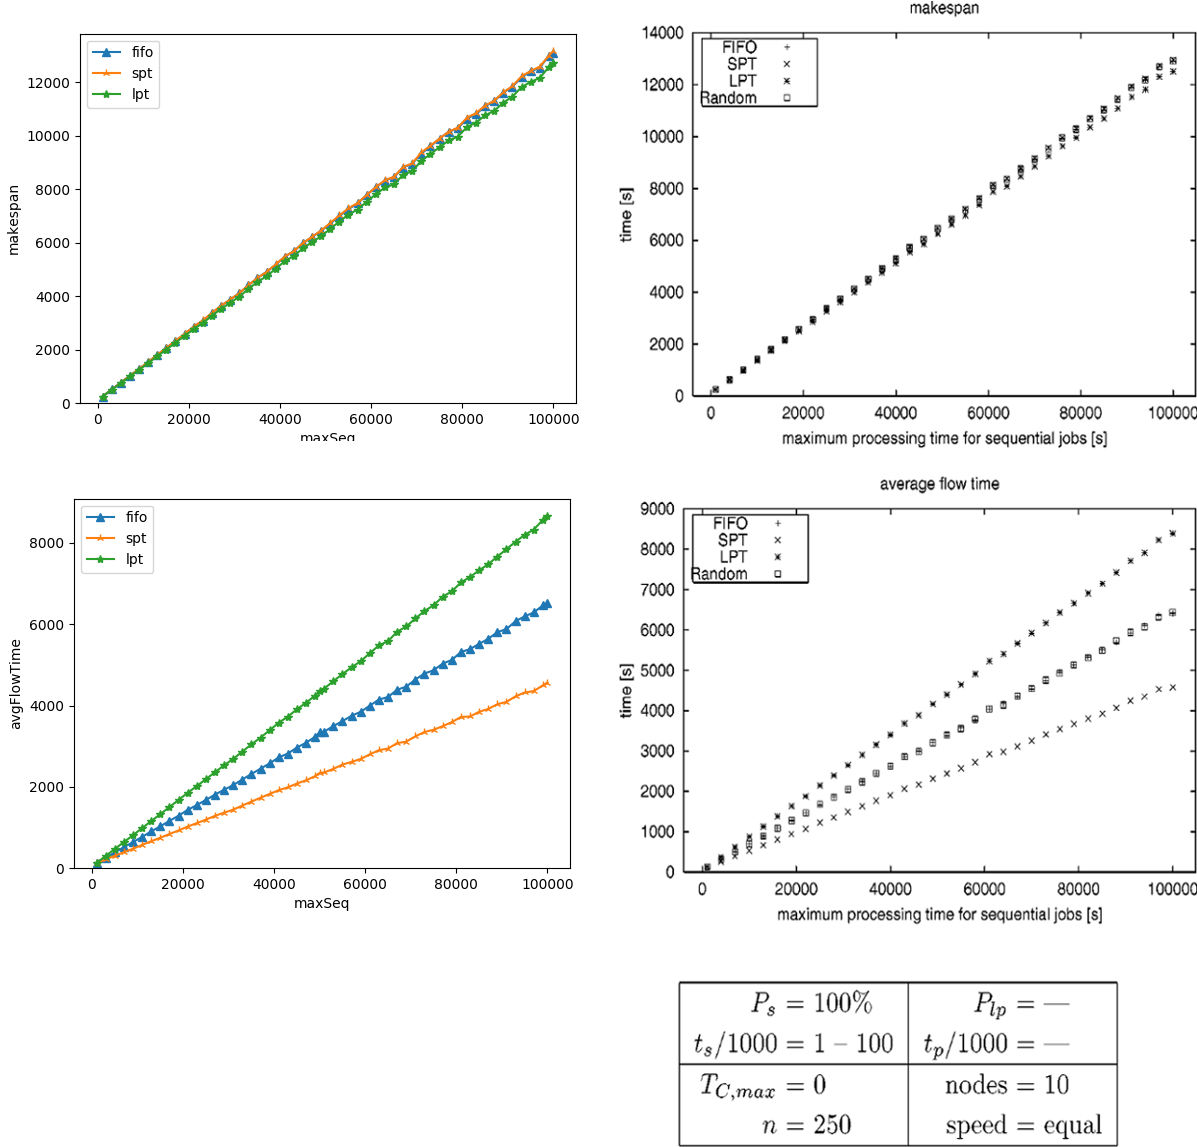
\includegraphics[width=\textwidth]{/home/hendrik/Programming/Python/BA/Docs/Hendrik/BA_Template/images/Figure_1.png}
\caption{Figure 1, Vergleich von Sequentiellen Aufträgen}
\label{figure1}
\end{figure}
\begin{figure}
	\centering
	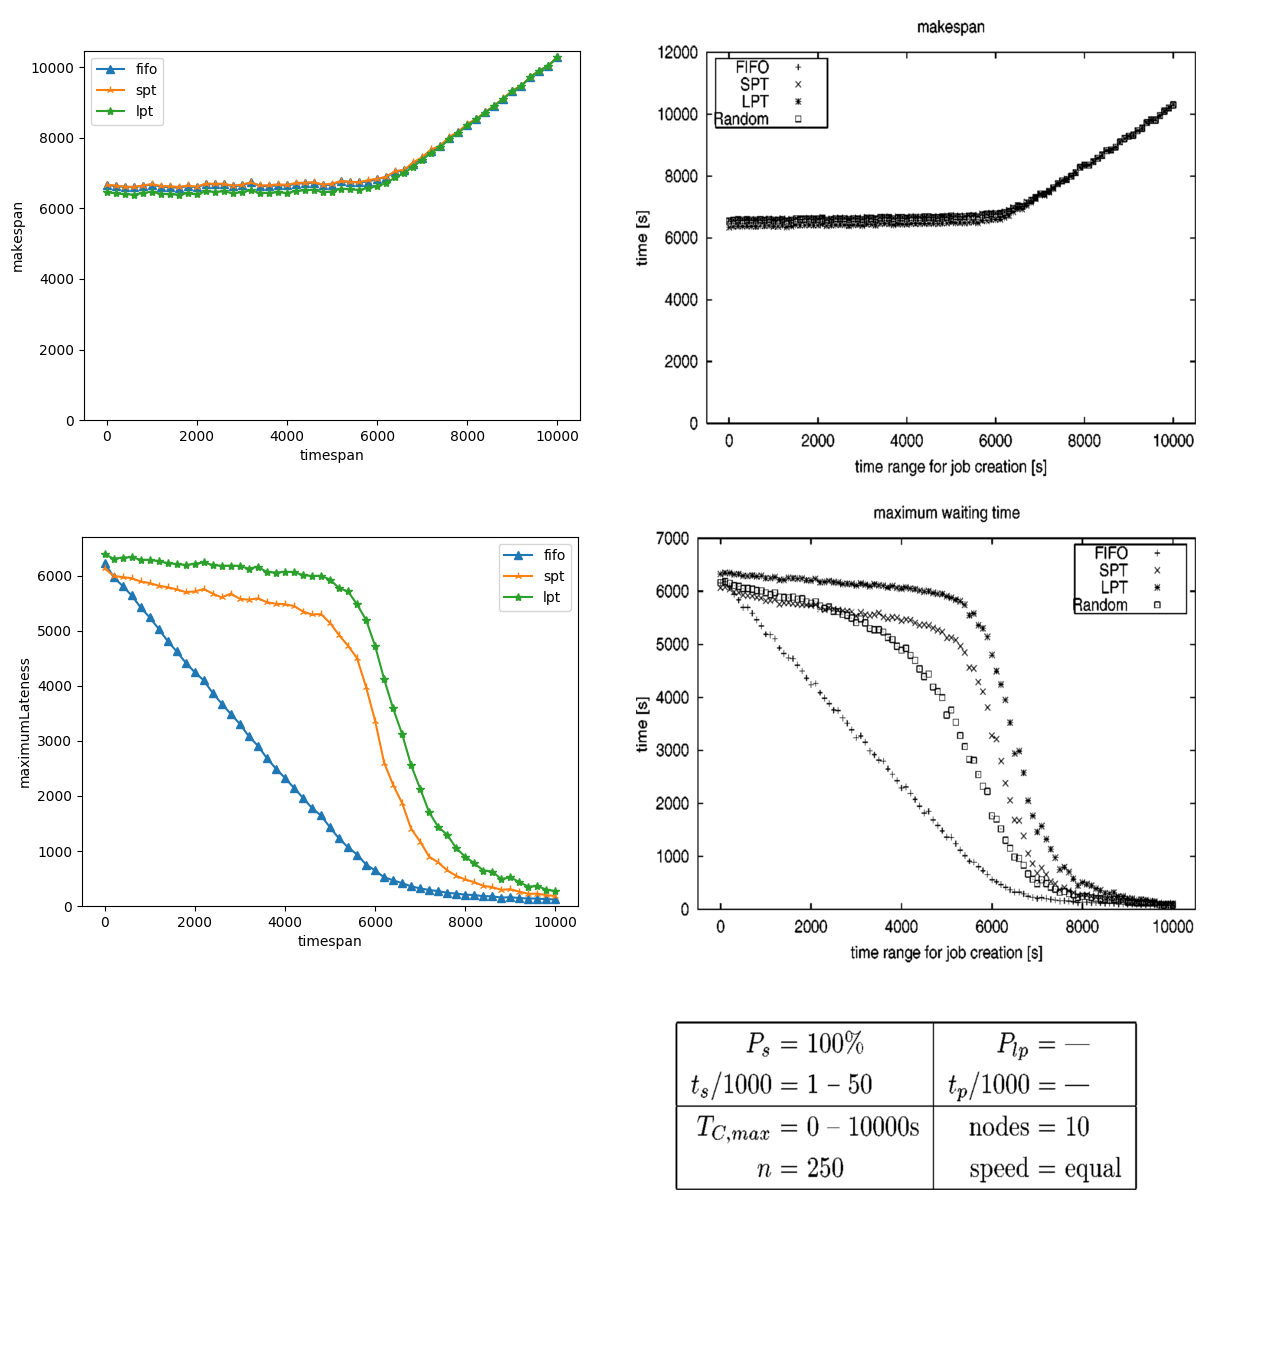
\includegraphics[width=\textwidth]{/home/hendrik/Programming/Python/BA/Docs/Hendrik/BA_Template/images/Figure_2.png}
	\caption{Figure 2, Vergleich von Sequentiellen Aufträgen, Erstellungszeit wird variiert5}
	\label{figure1}
\end{figure}
\begin{figure}
	\centering
	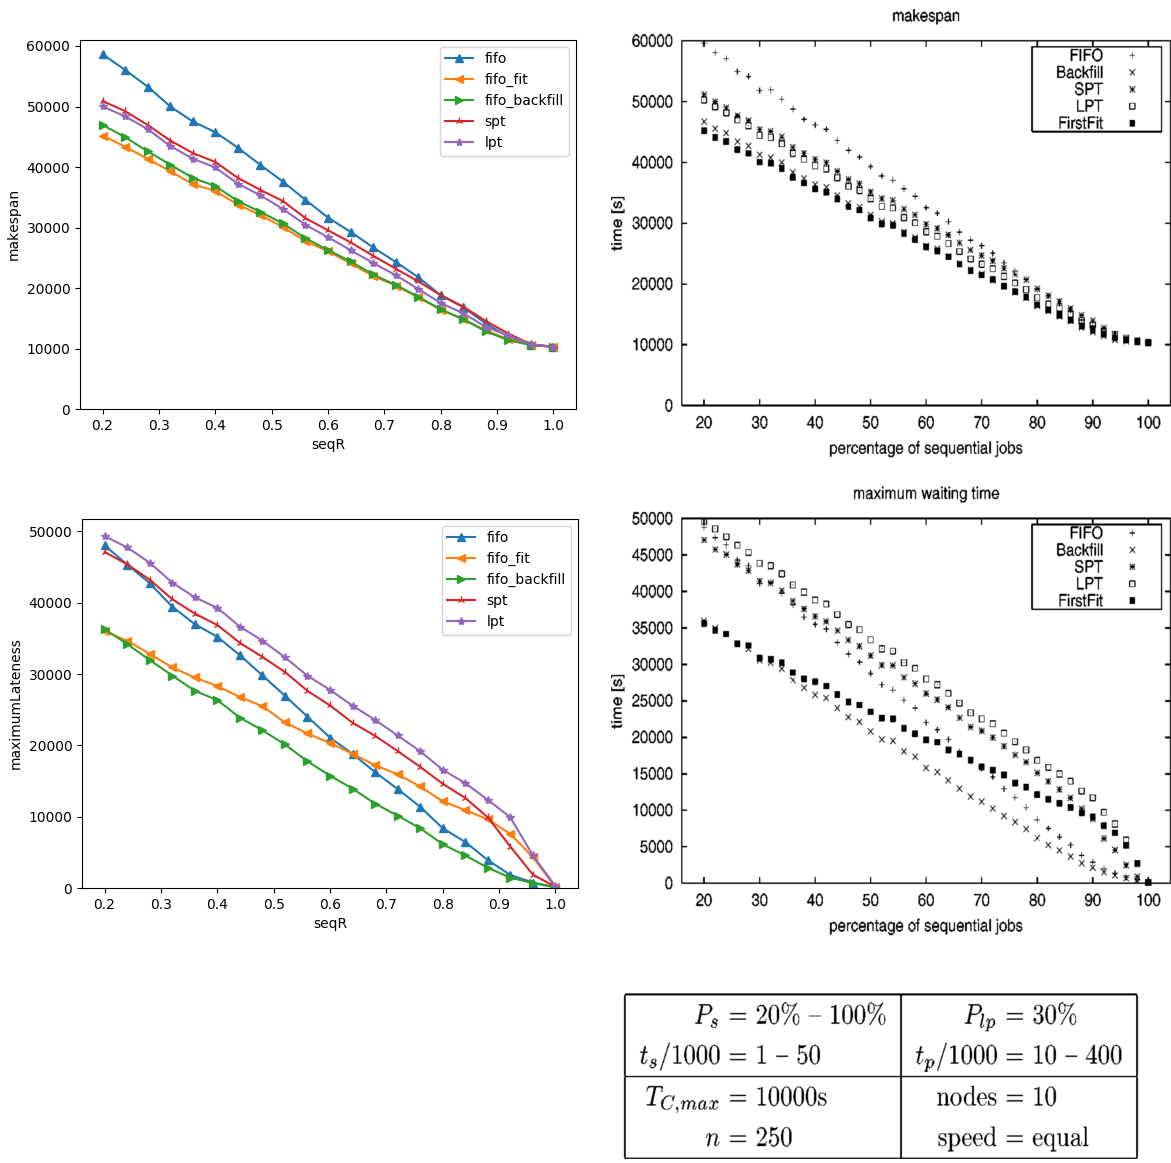
\includegraphics[width=\textwidth]{/home/hendrik/Programming/Python/BA/Docs/Hendrik/BA_Template/images/Figure_3.png}
	\caption{Figure 1, Vergleich von Sequentiellen Aufträgen}
	\label{figure3}
\end{figure}

\FloatBarrier

\subsubsection{Unterschiedlich schnelle Knoten ab Abbildung 4}
Ab dem vierten Experiment offenbart sich folgendes Problem: Die Geschwindigkeiten der Knoten variieren. Sie entsprechen den Messungen von "22 Knoten des lokalen Netzwerks". Jedoch werden diese gemessen Geschwindigkeiten weder in der besprochenen, noch in früheren Veröffentlichungen dargelegt (hier andere paper einfügen). Dies stellt eine sehr hohe Hürde zur Reproduktion dar.\\

\begin{figure}
	\centering
	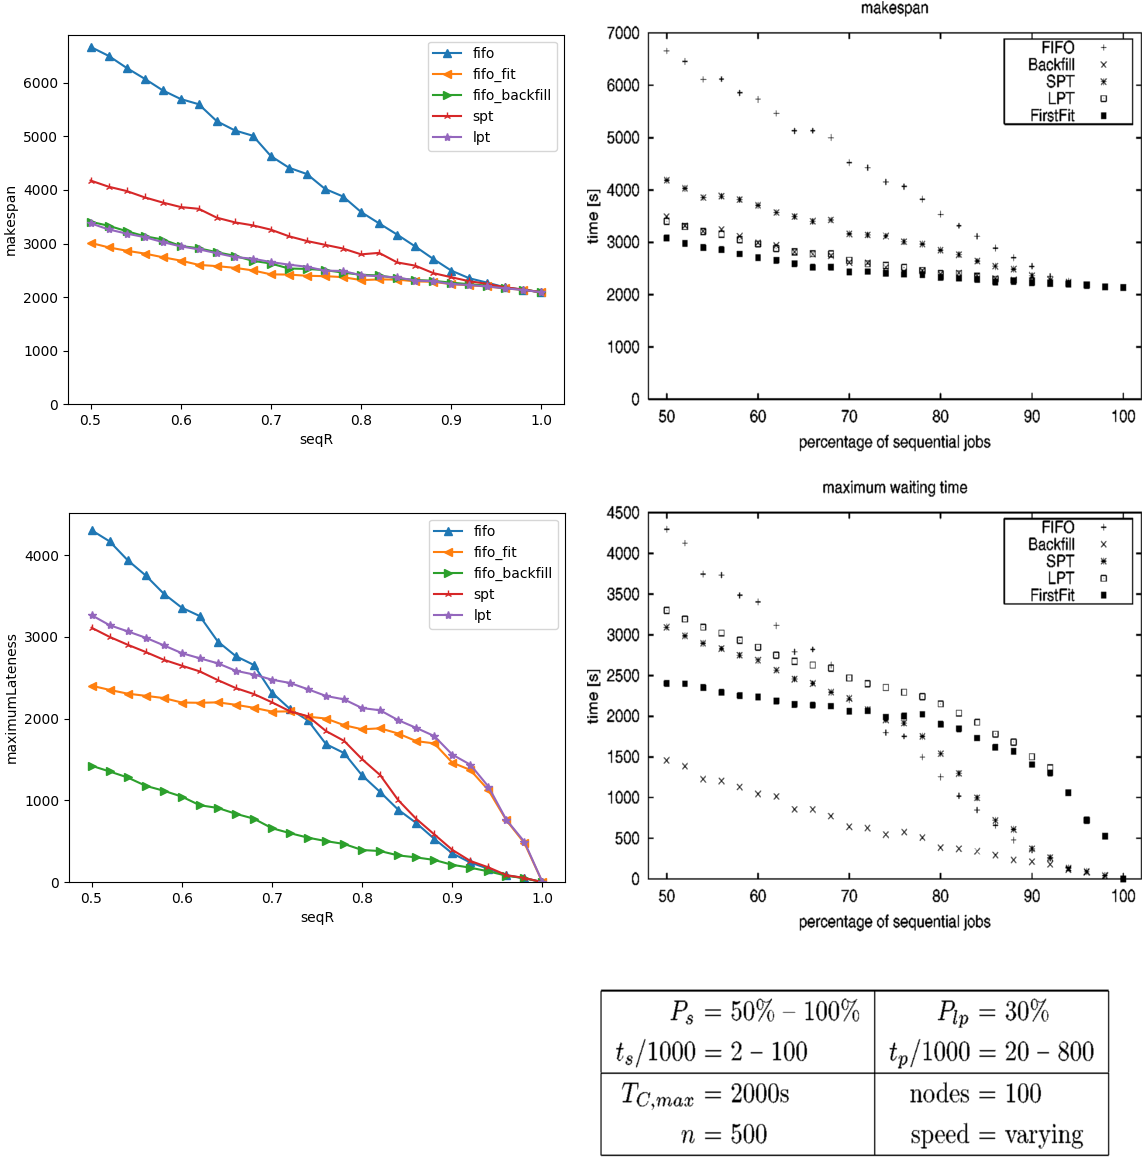
\includegraphics[width=\textwidth]{/home/hendrik/Programming/Python/BA/Docs/Hendrik/BA_Template/images/Figure_5}
	\caption{Unterschiedlich schnelle Knoten:\\
	75 Knoten mit Geschwindigkeit 275, 25 Knoten mit Geschwindigkeit 825}
	\label{figure5}
\end{figure}

Um die in \ref{chap:higher-order} vorgeschlagenen Scheduler auch in Eperimentaufbau 4 bis 9 antreten zu lassen, wird eine ungefähre Verteilung der Geschwindikeiten geschätzt.
Hier für wird Abbildung 5 \ref{figure5} herangezogen. In diesem Experiment wird die Bearbeitungsspanne (makespan) angegeben. Dadurch lässt sich eine untere Schranke für die gesamte Rechenleistung des Klusters finden. Wenn durch FirstFit jeder Knoten zu jedem Zeitpunkt ausgelastet wäre, müsste die durchschnittliche Rechenleistung aller Knoten im beschriebenen Versuchsaufbau 384 betragen. Dies wird am Wert für einen Auftragsmix aus 50\% sequentiellen Aufträgen abgelesen. 100 Knoten unbekannter Geschwindigkeit benötigen etwa 3000 Sekunden um 500 Aufträge mit einer durschnittlichen Bearbeitungszeit von 230500 Sekunden fertigzustellen. Um die durch die Algorithmen und die online eingehenden Aufträge entstehenden Effizienzeinbußen auszugleichen, wird die Geschwindigkeit der Knoten zusätzlich um 7,5\% erhöht.
\begin{align*}
\frac{250*(51* 10^3 + 410*10^3)*s}{100x} &= 3000s \\
\frac{250*461}{300} &= x
\end{align*}
Die Frage nach der Art der verwendeten Verteilung lässt sich nicht kären. Deswegen wird hier die einfachste Verteilung gewählt: 2 Klassen von Knoten, mit unbekannten Geschwindgkeiten und Anzahlen. Der zweidimensionale Lösungsraum kann durch eine weitere Annahme auf einen eindimensionalen Raum reduziert: Die Menge der langsamen Knoten soll die selbe Gesamtleistung besitzen wie die Menge der schnellen Knoten.\\
Dies führt zu einer größeren Anzahl langsamer und einer geringeren Anzahl schnellerer Knoten. Diese Konstellationen sind sicherlich interessanter als ihre Umkehrung. Gäbe es viele schnelle und wenige langsame Knoten, wären ähnliche Ergebnisse dadurch zu erreichen, die langsamen Knoten wegzulassen, wodurch sich die Situation nicht viel von den zuvor untersuchten unterscheiden würde.\\
Damit bleibt nur eine einzige Variable, der Anteil der langsamen Knoten im Klaster. Der Wert 0,75 erzeugt visuell vergleichbare Ergebnisse.

\FloatBarrier

\subsubsection{Experimente 4 bis 9}
Ab Experiment 4 kann keine Vergleichbarkeit der Modelle mehr sichergestellt werden. Trozdem werden die Versuche nachgestellt, um die Algorithmen in \ref{chap:higher-order} gegen die fünf bekannten antreten zu lassen. Die Auswertung kann in \ref{weiter} gefunden werden.


\section{Weiterführende Untersuchungen}
\label{weiter}

\begin{figure}	
	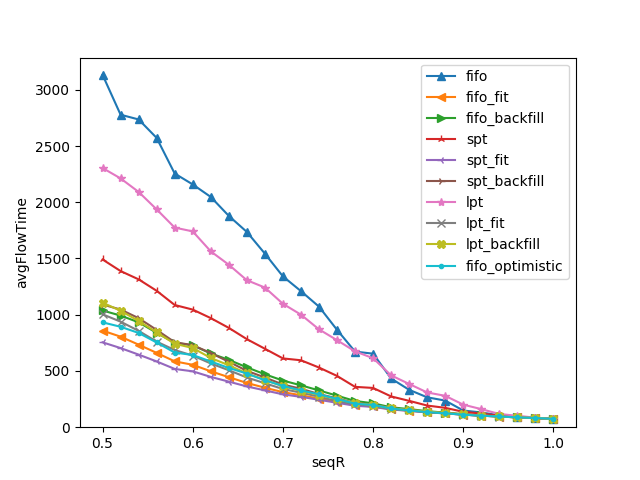
\includegraphics[width=\textwidth]{/home/hendrik/Programming/Python/BA/Docs/Hendrik/BA_Template/images/Figure_4_1}
	\caption{Varieren des Anteils von sequenziellen Aufträgen}
	\label{figure_4_1}
\end{figure}
\begin{figure}	
	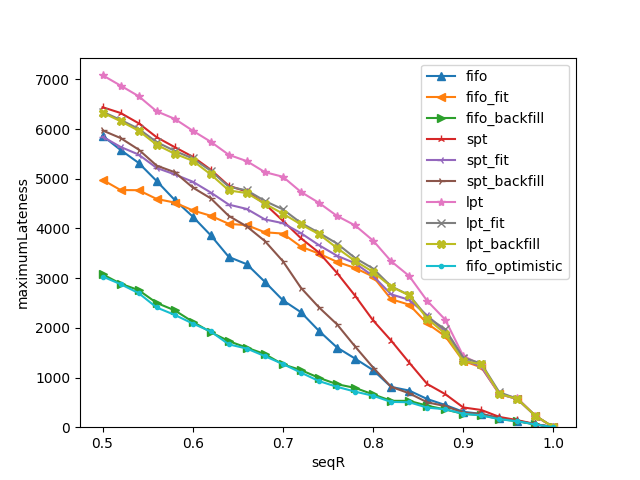
\includegraphics[width=\textwidth]{/home/hendrik/Programming/Python/BA/Docs/Hendrik/BA_Template/images/Figure_4_2}
	\caption{Varieren des Anteils von sequenziellen Aufträgen}
	\label{figure_4_2}
\end{figure}
\begin{figure}	
	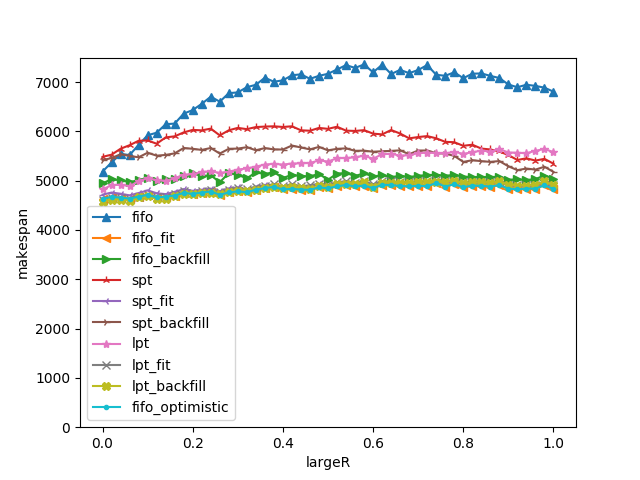
\includegraphics[width=\textwidth]{/home/hendrik/Programming/Python/BA/Docs/Hendrik/BA_Template/images/Figure_6_1}
	\caption{Varieren des Anteils von großen parallelen Aufträgen}
	\label{figure_6_1}
\end{figure}
\begin{figure}	
	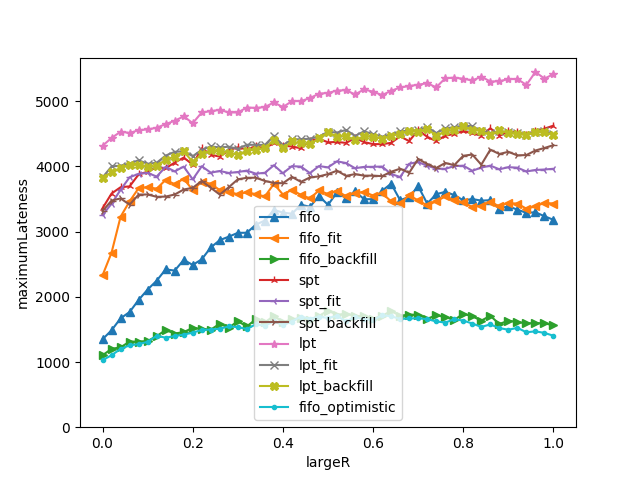
\includegraphics[width=\textwidth]{/home/hendrik/Programming/Python/BA/Docs/Hendrik/BA_Template/images/Figure_6_2}
	\caption{Varieren des Anteils von großen parallelen Aufträgen}
	\label{figure_6_2}
\end{figure}
\begin{figure}	
	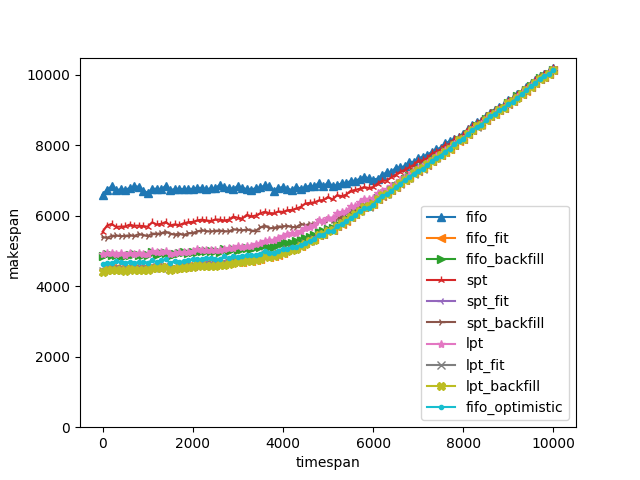
\includegraphics[width=\textwidth]{/home/hendrik/Programming/Python/BA/Docs/Hendrik/BA_Template/images/Figure_7_1}
	\caption{Varieren der Zeitspanne des Anmeldens von Aufträgen}
	\label{figure_7_1}
\end{figure}
\begin{figure}	
	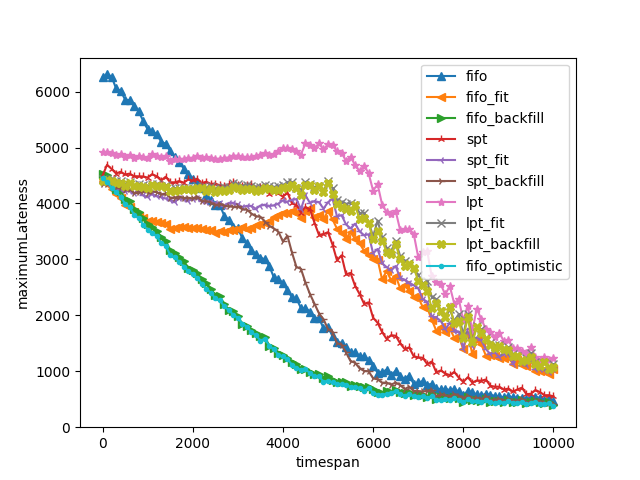
\includegraphics[width=\textwidth]{/home/hendrik/Programming/Python/BA/Docs/Hendrik/BA_Template/images/Figure_7_2}
	\caption{Varieren der Zeitspanne des Anmeldens von Aufträgen}
	\label{figure_7_2}
\end{figure}
\begin{figure}	
	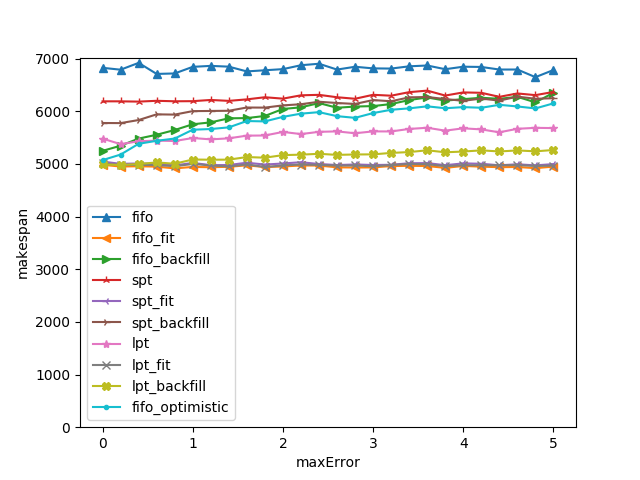
\includegraphics[width=\textwidth]{/home/hendrik/Programming/Python/BA/Docs/Hendrik/BA_Template/images/Figure_8_1}
	\caption{Varieren des erlaubten relativen Fehlers in der Angabe der Laufzeit}
	\label{figure_8_1}
\end{figure}
\begin{figure}	
	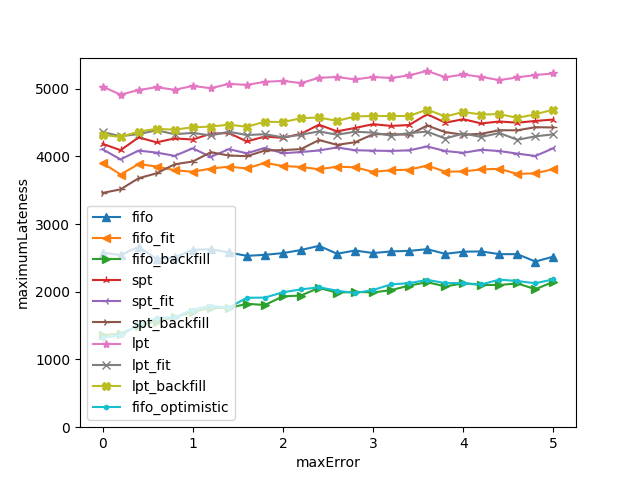
\includegraphics[width=\textwidth]{/home/hendrik/Programming/Python/BA/Docs/Hendrik/BA_Template/images/Figure_8_2}
	\caption{Varieren des erlaubten relativen Fehlers in der Angabe der Laufzeit}
	\label{figure_8_2}
\end{figure}


\FloatBarrier
\subsection{Backfilling und Fit als Funktionen höherer Ordnung}
\label{chap:higher-order}

Die in Kapitel 2 vorgestellten Funktionen FirstFit und Backfilling sind nur Abwandelungen der FiFo Funktion. Beide wählen den nächsten Auftrag abhängig vom Einreihungszeitpunkt $q_j$, jedoch unter Einschränkungen. "FiFo-Fit" wählt den ersten unter den startbaren Aufträgen aus, "FiFo-BackFilling" wählt den ersten Auftrag, oder einen, der den Bearbeitungsbeginn des ersten Auftrags nicht verzögert. "-Fit" und "-Backfilling" fügen also einen relevanten Kontext hinzu. Es liegt nahe, diese Erweiterungen als Funktionen höherer Ordnung zu betrachten. Ihre Domäne besteht aus einer Scheduling Funktion, den wartenden Aufträgen und einen Kontext - Anzahl an verfügbaren Knoten oder die Abschlusszeitpunkte und die Parallelität der laufenden Aufträge -, und bilden diese partiell auf einen Auftrag ab. 
Da FirstFit-Backfilling von [PaperZitat] als Sieger auserkohren wurde, LPT und GPT aber nicht im Backfilling Kontext untersucht wurden, wird im folgenden untersucht, ob LPT oder GPT mit -FirstFit oder -Backfilling ähnlich gute Ergebnisse erzielen können.\\
In \ref{proptest} wird eine Abwandlung des Backfillings vorgestellt, das optimistische Backfilling. Dieses wird hier auch mit untersucht, allerdings nur im FiFo Kontext.

\paragraph{SPT}
In Abbildung \ref{figure_4_1} wird die durschnittliche Zeit eines Auftrags im System gemessen. Dabei schneidet SPT-Fit besser ab als alle anderen Algorithmen. Den zweiten Platz belegt FiFo-Fit. Für die durschnittliche Systemzeit ist es wichtig, so schnell wie möglich Aufträge fertig zu stellen. Deshalb eigenen sich ''-Fit'' Funktionen, besonders in Kombination mit SPT. Erstaunlicherweise ist ''-Fit'' jedoch im Bezug zur Systemzeit nicht vollständig monoton. So gilt für die Messungen zwar SPT $<$ LPT $<$ FiFo, jedoch Fit$($FiFo$)$ $<$ Fit$($LPT$)$.\\
In Abbildung \ref{figure_7_2} erzielt SPT-Fit die selben Werte wie FiFo-Fit und LPT-Fit. In diesem Experiment wird die Bearbeitungsspanne in Abhängigkeit von einer relativen Fehlerrate in der Angabe von Bearbeitungszeiten ermittelt.\\


\paragraph{LPT}
In Abbildung \ref{figure_6_1} gibt es eine Klasse an Algorithmen, die gleich gute Ergebnisse erzielen. Darunter FiFo-Fit, SPT-Fit, LPT-Fit, LPT-Backfill und FiFo-Optimistic-Backfill. In diesem Experiment wird die Bearbeitungsspanne in Abhängigkeit des anteils von großen parallelen Aufträgen gemessen. LPT-Fit ist hier deshalb eine gute Wahl, da LPT im Vergleich zu SPT und FiFo für eine geringere Spanne sorgt (vgl. auch \ref{figure3}). ''-Fit'' und ''-Backfill'' sorgt dafür, dass lange Phasen zum Anfang des Laufs, in denen einige Knoten nicht genutzt werden, während lange Aufträge abgearbeitet werden, gefüllt werden können.\\
Diese Beobachtung wiederholt sich in Abbildung \ref{figure_7_1}. Auch hier wird die Bearbeitungsspanne als Maß angelegt.\\

\paragraph{Optimistisches Backfilling}
Dieser Algorithmus wird in \ref{optfill} vorgestellt.\\
Beim Optimistischen Backfilling stellt sich vorallem die Frage, wie groß der Unterschied zum ''normalen'' Backfilling ist, und ob es ein Unterschied zu unseren Gunsten ist. Hierfür wurde nur FiFo in beiden Kontexten herangezogen.\\
In \ref{figure_4_1} bietet das Optimistische Verfahren einen leichten, jedoch erkennbaren Vorteil Hier wird die durchschnittliche Systemzeit von Aufträgen in Abhängigkeit des Anteils sequentieller Aufträge ermittelt. Es erscheint nachvollziebar, dass, vorausgesetzt es gibt etwa gleich viele sequezielle als auch parallele Aufträge, eine Leistungssteigerung durch das Optimistische Verfahren erzielt werden kann. Da dieses weniger restriktiv ist, welche Aufträge gestartet werden dürfen, um Lücken zu füllen.\\
So auch in \ref{figure_7_1}. Hier wird die gesamte Bearbeitungszeit in Abhängigkeit eines erlaubten Fehlers untersucht. Die selbe Argumentation erscheint plausibel. Wenn die Bearbeitungszeit eines Auftrags nicht korrekt angegben wurde, werden weniger Aufträge gestartet um Lücken zu füllen. Das Optimistische Backfilling darf trotzdem Aufträge die wenige Knoten benötigen starten, und nutzt so die Freiräume besser aus.\\
In allen anderen Versuchen ist kein nennenswerter Unterschied feststellbar. Es erscheit, als wären die in \ref{optfill} genannten Konstellationen selten genug, als dass sie die nicht genutzten Chancen des ''normalen'' Backfilling überwiegen. Zumindest in den hier untersuchten Experimenten lässt sich die optimistische Variante als Ersatz empfehlen. In den meisten Fällen ist kein deutlicher Unterschied erkennbar, aber wenn, dann immer zu unseren Gunsten. Die Auswirkung auf LPT und SPT könnten in Zukunft untersucht werden. 

\FloatBarrier

\subsection{Property Based Testing zum Erkenntnisgewinn}
\label{proptest}
\paragraph{Testen statt Simullieren}
Während das Simullieren des Rechenclusters gute Auskunft darüber gibt, wie sich das System bei einer langen Reihe an Aufträgen verhällt, kristalliesiert sich dabei lediglich das durchschnittliche Verhalten heraus. Obwohl diese Analyse sinnvoll ist, um verschiedene Scheduling Funktionen asymptotisch mit einander zu vergleichen, wird durch das Mitteln von hunderten von Läufen nicht ersichtlich, in welchen Fällen eine normalerweise unterlegene Scheduling Funktion einer Anderen überlegen ist.\\
Um eine Intuition für die Unterschiede zwischen Scheduling Funktionen entwickeln zu können ist es hilfreicher, die durch kleinstmögliche Listen an Aufgaben erzeugten Läufe zu vergleichen. Um diese minimalen Beispiele zu generieren, kann ein Property Based Testing Framework verwendet werden. Ein guter Einstiegspunkt in dieses Thema ist [initial Paper 1999]. Hier nur eine kleine Zusammenfassung der für uns wichtigen Aspekte. \\
Ein Test besteht aus einer zu testenden Funktion, eine Eigenschaft, die die Ausgabe der Funktion haben soll, und einem Generator, der Eingaben produziert. Sobald eine Eingabe gefunden wird, deren Ausgabe die geforderte Eigenschaft nicht erfüllt, wird die Eingabe automatisch geschrumptf. Dies führt zu einem leichter interpretierbaren Beispiel, da der ausgegebene Fall "kein Rauschen" enthällt.
Eine Zahl wird geschrumpt, in dem sie verringer wird, ein Tupel von Zahlen, in dem eines der Elemente geschrumpft wird, und eine Liste, in dem Elemnter der Liste weggelassen oder geschrumpft werden.\\
Um ein minimales Beispiel zu finden, in dem Scheduling Funktion $S_1$ Ziel Funktion $T$ besser minimiert als Scheduler $S_2$, können wir die Eigenschaft $T(S_1(x)) >= T (S_2(1))$, mit einem Auftragsgenerator$X$: $(Anzahl Konten,[(\pi_j <= Anzahl Knoten,p_j,q_j)])$ überprüfen.
Ein vom Testframework gefundenes minimales Gegenbeispiel, zeigt uns einen Speziellen Fall, in dem $S_1$ ein besseres Ergebnis erzielt als $S_2$
Für die meinsten Scheduling Funktionen ist das minimal Beispiel eines mit 3 Aufträgen, und einer kleinen Anzahl an Knoten [genaues nochmal testen].

Hier nun einige Beispiele:\\

\paragraph{Optimistisches Backfilling}
\label{optfill}
Das vorgestellte ''-Backfilling'' Verfahren wirkt auf den ersten Blick zurückhaltend. Das angegebene Ziel, die zum ''-Fit'' verglichene Wartezeit gering zuhalten, wird erfüllt, in dem große Aufträge nicht benachteiligt werden. Kleine werden nur vorgezogen, wenn sich dadurch die Wartezeit des besten, aber nicht startbaren Kandidaten, nicht verzögert. Dies wird erreicht, in dem ein Auftrag $P'$ nur starten darf, wenn er abgeschlossen wird, bevor der beste Kandidat $P$ startet.\\
Warum aber darf ein Auftrag $P'$, der wenige Knoten benötigt, nicht starten, vorausgesetzt, er nimmt nur so wenige Knoten in Anspruch, dass $P$ wie geplant starten kann ($P$ benötigt noch $n$ Knoten zum starten, sobald er starten wird, sind aber $n+k, k>0$ Knoten frei, und $\pi_{P'} <= k$).\\
Es ist intuitiv, des es einen Haken gibt. Ohne in Scheduling Theorie geübt zu sein, ist es aber nicht einfach, aus dem Stand ein Beispiel zu konstruieren, in dem sich das optimistische -Backfilling negativ auf die Wartezeit auswirkt. Allerdings kann dank Property Based Testing ohne viel Mühe eines in wenigen Sekunden generiert werden.

\begin{figure}
\centering
\begin{verbatim}
Is fifo\_optimistic allways better than fifo\_backfill by maximumLateness?
No! counterexample:
queueintT, processingT, realProcessingT, degreeOfParallelism
id: 0, qT: 1, pT: 3, rPT: 3, doP: 1
id: 1, qT: 0, pT: 3, rPT: 3, doP: 2
id: 2, qT: 0, pT: 1, rPT: 1, doP: 2
id: 3, qT: 0, pT: 1, rPT: 1, doP: 3

maximumLateness of fifo\_optimistic: 4
[0]:112-3
[1]:112-3
[2]:-0003

maximumLateness of fifo\_backfill: 3
[0]:1123---
[1]:11-3000
[2]:--23---
\end{verbatim}
\caption{Vergleich vom Normalem und Optimistischem Backfilling}
\label{onlateness}
\end{figure}

\FloatBarrier

Hier ist der Optimistische Algorithmus zu vorfreudig. Auftrag 0 wird gestartet, obwohl er (als einziger) nicht seit beginn angemeldet ist. Dadurch wird Auftrag 3 nach hinten geschoben, und die maximale Wartezeit für 3 steigt. Trozdem is die Auslastung des optimistischen Algorithmus deutlich besser. Der findet man auch einen Fall, in dem sowohl die maximale Verspätung, als auch die gesamt Bearbeitungszeit schlechter sind?\\


\begin{figure}
\centering
\begin{verbatim}
Is fifo_optimistic allways better than <function System.fifo_backfill at 0x7f42574fd7b8> by <function maximumLateness at 0x7f42408ff400> ?
No! counterexample:

queueintT, processingT, realProcessingT, degreeOfParallelism
id: 0, qT: 1, pT: 1, rPT: 1, doP: 4
id: 1, qT: 1, pT: 3, rPT: 3, doP: 1
id: 2, qT: 1, pT: 3, rPT: 3, doP: 1
id: 3, qT: 0, pT: 4, rPT: 4, doP: 3
id: 4, qT: 0, pT: 1, rPT: 1, doP: 2

maximumLateness offifo_optimistic: 4
makespan of fifo_optimistic: 8
[0]:334-0---
[1]:334-0---
[2]:33--0222
[3]:-1110---

maximumLateness offifo_backfill: 3
makespan of fifo_backfill: 7
[0]:3340---
[1]:33-0111
[2]:33-0222
[3]:--40---
\end{verbatim}
\caption{Vergleich vom Normalem und Optimistischem Backfilling in Spanne und Verspätung}
\label{onlatenessmakespan}
\end{figure}

Natürlich. Auch hier kann ein durch Property Based Testing ein Fall konstruiert werden. Allerdings besteht hier das kleinste gefundene Beispiel bereits aus 5 Aufträgen. Es ist also zu erwarten, dass solche Konstellationen selten genug sind. Eine genauere Untersuchung dazu im Abschnitt \ref{chap:higher-order}
Dauert ca ne Minute auf crappy laptop\\
\FloatBarrier

Wie in der Grafik \ref{onlateness} nach einem Schritt erkennbar, benachteiligt ein solcher optimistisch gestarteter langer, kleiner Auftrag nicht den besten Kandidaten (Auftrag 4), allerdings den zweitbesten Kandidaten (Auftrag 0). Ob dies ein seltener Fall ist, oder ob sich Optimismus im Mittel auszahlt, kann wiederum durch eine Statistische Asuwertung untersucht werden.\\

Außerdem ist es interessant zu beobachten, welche Informationen implizit aus diesem Gegenbeispiel gezogegen werden können. Zum Beispiel, dass im ersten Lauf \ref{onlateness} nur ein einziger online Auftrag (d.h. nicht schon zum Zeitpunkt 0 bekannt) nötig ist, aber um das optimistische Verfahren in beiden Metriken zu schlagen, werden 3 online Aufträge sowie ein zusätzlicher Auftrag benötigt. Es fällt auch auf, dass in diesem Beispiel FiFo-Backfill nie vom Backfilling Gebrauch macht. Es verhällt sich immer wie das blanke FiFo Verfahren. 
Des weiteren fällt auf, dass das Shrinking Verfahren herausgefunden hat, dass zur Berechnung der Laufzeiten von parallelen Aufträgen hochgerundet wird (s. \ref{spt-lpt-time}). Da dies der Lesbarkeit der Tests zuwider läuft, kann die Bearbeitungszeit jedes Auftrags einfach auf das nächste Vielfache der Parallelität gesetzt werden.

dadurch gefunden: nach QT als optimisierung zu sortieren reicht nicht, auch hier nach id mit

\subsection{Simulation von Fehlerhaftem Verhalten}
\label{simErrors}

\paragraph{Lorem}
ipsum
\chapter{Fazit}

\paragraph{Scheduling Funktionen höherer Ordnung}
Die Sichtweise der Funktionalen Programmierung auf Scheduler ist offensichtlich nützlich. Arndt et al. \cite{Arn99} haben zurecht den Backfilling Algorithmus als bevorzugten Scheduler gewählt.
5 + 3*(5*5) = 80 algos (wenn true spt und true lpt zählen)

\paragraph{Vergleich von Simulation und Testing}
Es ist fraglich, wieweit die Methode des kleinsten Falles, in dem ein Algorithmus gegen gegen einen anderen die Oberhand gewinnt, für die Analyse der verschiedenen Leistungen taugt. Sicherlich ist sie ein sehr nützliches Hilfsmittel, das neue Einsichten gewähren kann. Sich schnell darüber klar werden zu können, in welchen Situation ein (ausgeklügelter) Algorithmus wie das Backfilling sich selbst überlistet, ist sicherlich eine gute Möglichkeit die eigene Intuition weiterzuentwickeln.\\
Zumal ist diese Methode beinahe ohne zusätzlichen Aufwand nutzbar. Bereits wenige Zeilen Code erlauben Einblicke in das Verhalten des Systems. Die eigentlichen Kosten dafür sind das wählen einer Ereignis orientieren Simulation. Eine Prozess orientiere Sichtweise führt dazu, dass das simulierte System näher am tatsächlichen System ist. Effekte, die natürlich durch parallel agierenden Agenten entstehen, wie etwa kritische Wettlaufsituationen, bekommt man ohne zusätzlichen Aufwand; ob nun gewünscht oder ungewünscht. Diese Effekte können durch eine zufällige Ausführungsreihenfolge mit simuliert werden, dies war allerdings nicht nötig, um vergleichbare Ergebnisse zu erzielen.

großes interesstes Kreuzprodukt


\paragraph{Lorem}
irgendwas zum pbt

ipsum


code??

% -------------------------------------------------------------------
% Appendix
% -------------------------------------------------------------------
%\include{appendix}
% -------------------------------------------------------------------
% Quellen
% -------------------------------------------------------------------
\cleardoublepage
%\bibliographystyle{IEEEtran}
\bibliographystyle{alphadin}
\bibliography{literatur}

% -------------------------------------------------------------------
\end{document}
% -------------------------------------------------------------------
